\documentclass[xcolor=x11names,t]{beamer}
\usefonttheme[onlymath]{serif} %Letras bonitas para las ecuaciones
\usepackage[utf8]{inputenc}
\usepackage[spanish]{babel}
\decimalpoint %para que la separacion de decimales sea con un punto 
\usepackage{amsfonts}
\usepackage{amsmath}
\usepackage{amssymb}
\usepackage{ragged2e}
\usepackage{wrapfig}
\usepackage{graphicx} % Allows including images
\usepackage{booktabs} % Allows the use of \toprule, \midrule and \bottomrule in tables

\usepackage[backend=bibtex,
            style=iso-numeric,
            autocite=plain,
            maxbibnames=3,
            maxcitenames=1,
            urldate=long,
            uniquelist=false
]{biblatex}

\addbibresource{biblio.bib}

%Tema madrid
\usetheme{Madrid}
%Circulos en los itemize
\useinnertheme{circles}

\setbeamertemplate{footline}[page number] % To replace the footer line in all slides with a simple slide count uncomment this line
\setbeamertemplate{navigation symbols}{} % To remove the navigation symbols from the bottom of all slides uncomment this line

\justifying
\definecolor{MediumGreen}{rgb}{0.36862, 0.66666, 0.65882}
\definecolor{InvisibleGreen}{rgb}{0.9, 0.92, 0.9}
\definecolor{InvisibleBlue}{rgb}{0.9, 0.9, 0.92}
\definecolor{MediumBlue}{rgb}{0.01176, 0.31372, 0.43529}
\definecolor{whitetxt}{RGB}{255,255,255}
\definecolor{bluewhite}{RGB}{134, 165, 202}
\definecolor{colorusach}{RGB}{0, 164, 153}
\definecolor{azulusach}{RGB}{0, 51, 146}
\definecolor{bodyexample}{RGB}{191, 223, 223}
\definecolor{titleexample}{RGB}{0, 127, 127}
\definecolor{alerblockcolortitle}{RGB}{235, 119, 4}
\definecolor{alerblockcolorbody}{RGB}{255, 223, 191}
\definecolor{InvisibleRed}{rgb}{0.92, 0.9, 0.9}
\definecolor{MediumRed}{rgb}{0.92549, 0.34509, 0.34509}
%Bloques redondos y con sombras
\setbeamertemplate{blocks}[rounded][shadow=true]

%Color de los titulos
\setbeamercolor{frametitle}{bg=colorusach,fg=whitetxt}
%Color del titulo principal (Primera página)
\setbeamercolor{title}{fg=whitetxt, bg=colorusach}
%Color parte de abajo
\setbeamercolor{author in head/foot}{bg=azulusach}
\setbeamercolor{title in head/foot}{bg=azulusach}
\setbeamercolor{date in head/foot}{bg=azulusach}

%color bloque de ejemplo
\setbeamercolor{block title example}{bg=colorusach}
\setbeamercolor{block body example}{bg=InvisibleGreen}

\setbeamercolor{block title}{bg=MediumBlue}
\setbeamercolor{block body}{bg=InvisibleBlue}
%Color bloque alerta
\setbeamercolor{block title alerted}{bg=MediumRed}
\setbeamercolor{block body alerted}{bg=InvisibleRed}




\usepackage{tikz}

%%%%%%%%%%%%%%%%%%%%%%%%%%%%%%%%%%%%%%%%%%%%%%%%%%%%%%%%%%%%%


\title{\textbf{Open Robotics}}
\subtitle{\textbf{Trabajo: Control de turtlesim con Arduino}}
\author{\textbf{Estudiante: René Torres \\ Profesor: José Pascal}}


\institute[DIMEC]{Universidad de Santiago de Chile \\
Carrera: Ingeniería Civil en Mecánica \\
e-mail: rene.torres.a@usach.cl, jose.pascal@usach.cl}

\begin{document}


\begin{frame}
    \begin{center}
        
\includegraphics[scale=0.23]{images/DIMECLOGO.png}      
    \end{center} 
    \maketitle
\end{frame}

\begin{frame}{Índice}
    \tableofcontents    
\end{frame}

\begin{frame}{Introducción}
    \section{Introducción}  
        \subsection{¿Qué es ROS?}
        \begin{block}{¿Qué es ROS?}
            Robot Operating System es un conjunto de librerías de software y herramientas, de código abierto (open source) que ayudan a desarrolladores de todo el mundo a construir aplicaciones robóticas.
        \end{block} 
       \begin{figure}
        \centering
        
\includegraphics[scale=0.1]{images/Ros_logo.png}
        \caption{Robot Operating System.}
        \label{fig:turtlesim}
    \end{figure}
\end{frame}

\begin{frame}{Objetivos}
    \section{Objetivos}  
    \begin{block}{Objetivo general}
        \subsection{Objetivo general}
        Controlar el movimiento de la tortuga de turtlesim con hardware a través de Arduino.
    \end{block}

    \subsection{Objetivos específicos}
    \begin{block}{Objetivos específicos}
        \begin{itemize}
            \item Aplicar los fundamentos de ROS en una aplicación práctica.
            \item Utilizar el protocolo de comunicación ROS serial con Arduino.
            \item Generar un archivo launch para ejecutar la aplicación.
        \end{itemize}
    \end{block}
\end{frame}



\begin{frame}{Diagrama de conexiones}
    \section{Desarrollo}
    \subsection{Diagrama de conexiones}
    \begin{figure}
        \centering
        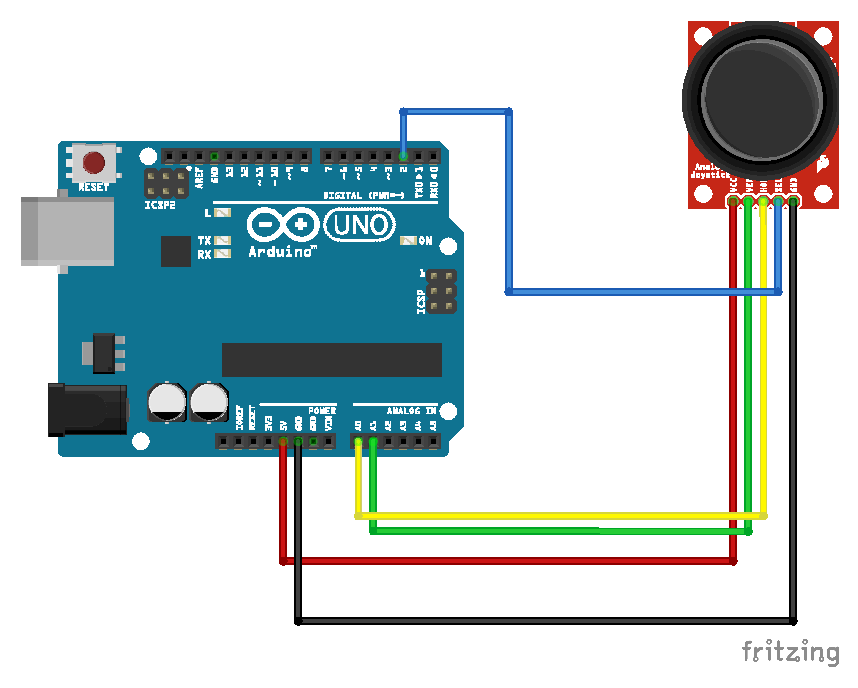
\includegraphics[scale=0.6]{images/diagrama_conexiones.pdf}
        \caption{Diagrama de conexiones.}
        \label{fig:conexiones}
    \end{figure}
\end{frame}

\begin{frame}{Módulo Joystick}
    \subsection{Módulo de joystick}
    \begin{figure}
        \centering
        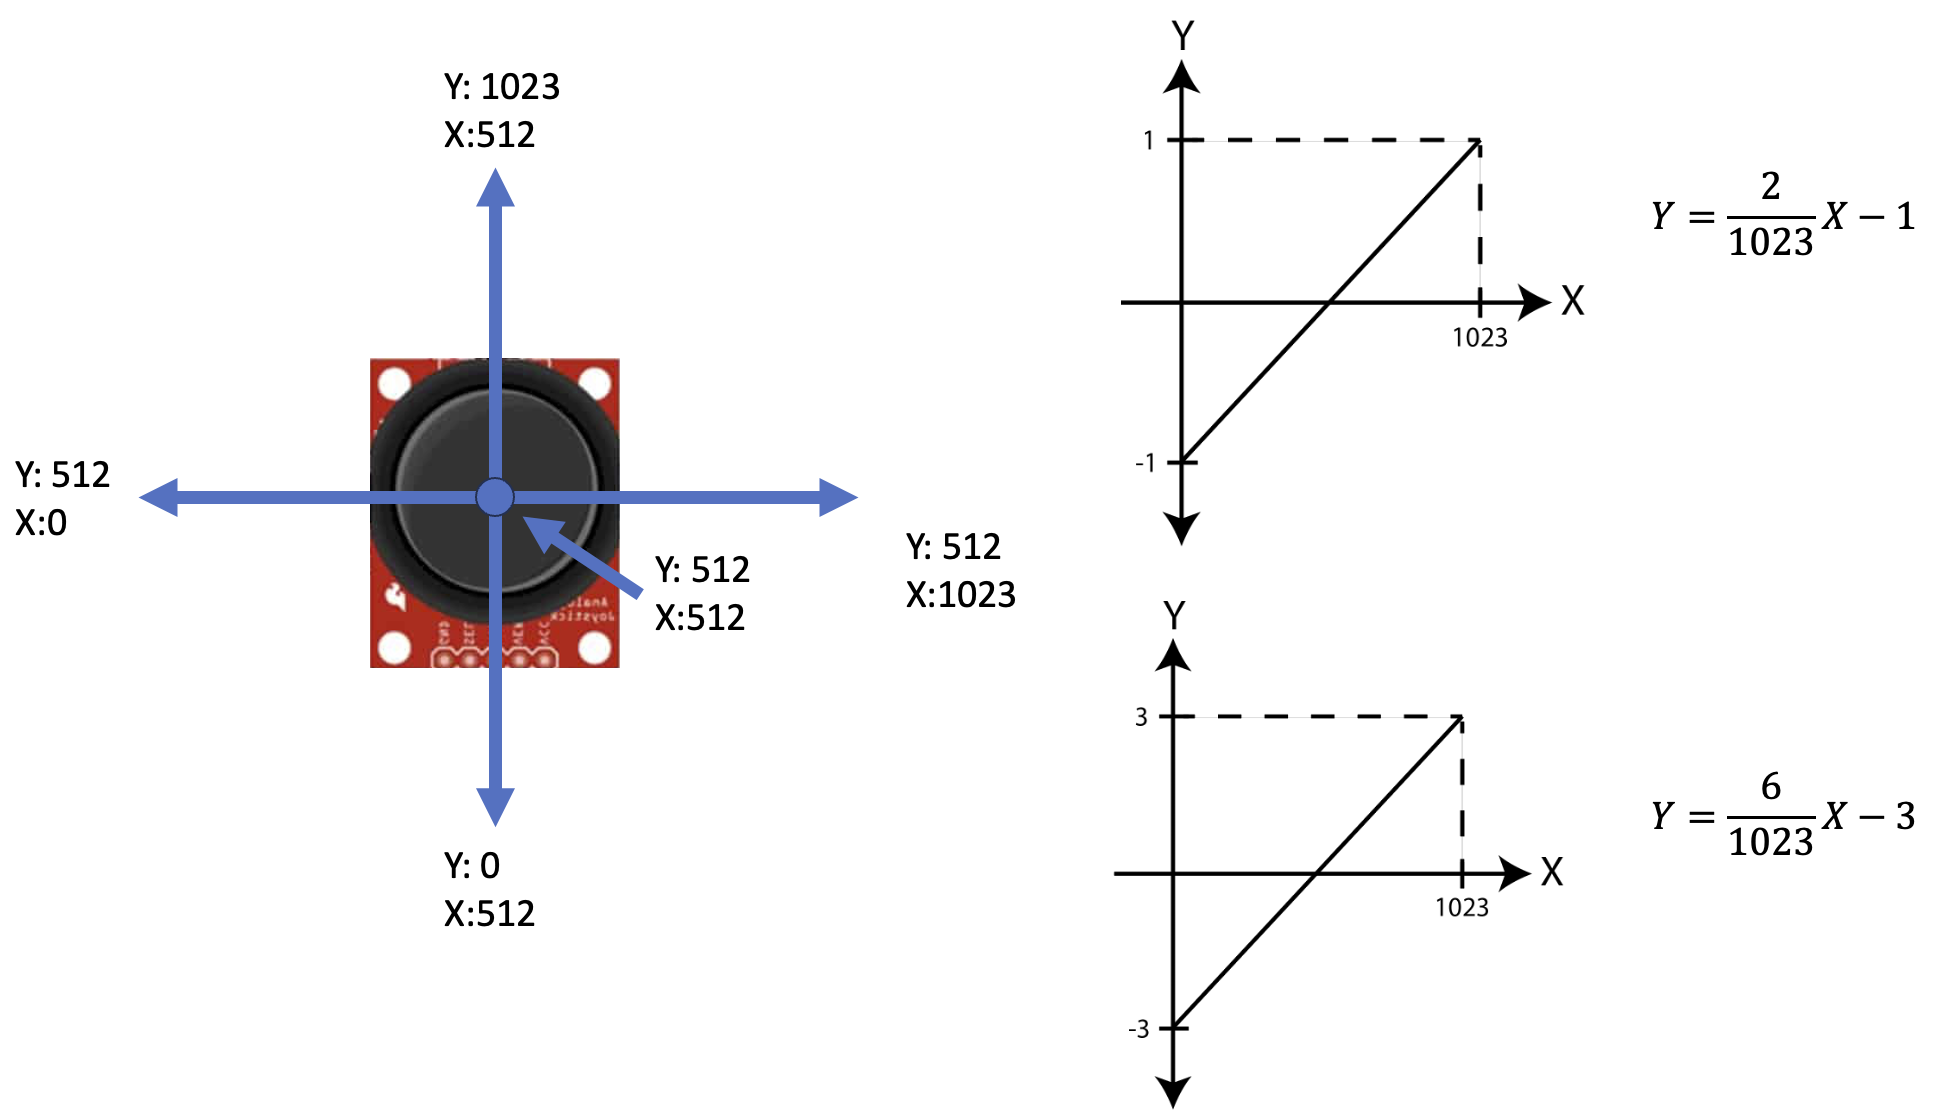
\includegraphics[scale=0.35]{images/rangojst.png}
        \caption{Transformación valores de joystick.}
        \label{fig:jstk}
    \end{figure}
\end{frame}

\begin{frame}{Diagrama de nodos de ROS}    
    \subsection{Diagrama de nodos de ROS}
    \begin{figure}
        \vspace{1.5cm}
        \centering
        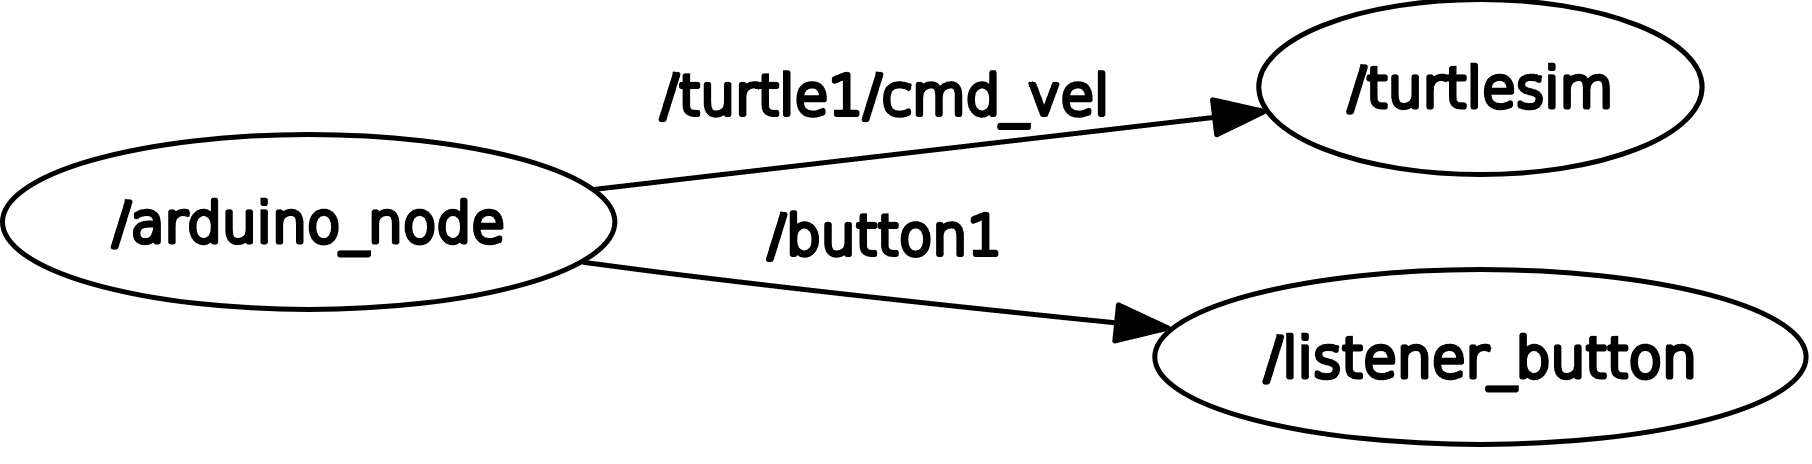
\includegraphics[scale=0.25]{images/rqtgraph.png}
        \caption{Diagrama de nodos de ROS.}
        \label{fig:rqtgraph}
    \end{figure}
\end{frame}

\begin{frame}{Funcionamiento de la aplicación}
    \subsection{Funcionamiento de la aplicación}
    \begin{figure}
        \centering
        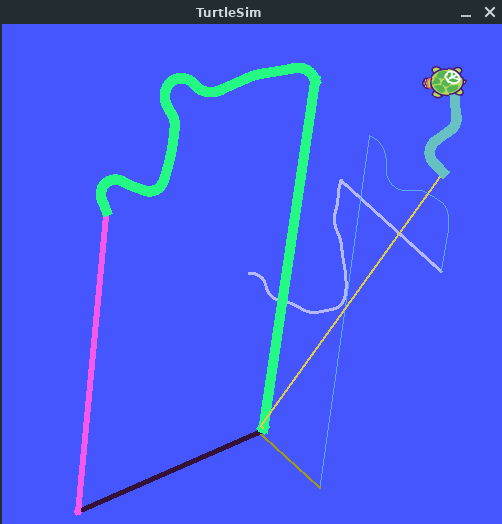
\includegraphics[scale=0.45]{images/turtlesim.png}
        \caption{Turtlesim.}
        \label{fig:turtlesim}
    \end{figure}
\end{frame}
    

\begin{frame}{Conclusiones}
    \section{Conclusiones} 
    \begin{itemize}
        \item Se logró controlar el movimiento de la tortuga de turtlesim mediante un modulo de Joystick a través de Arduino con ROS.
        \item Se aplicaron los fundamentos de ROS en una aplicación práctica, creando nodos publicadores y subcriptores.
        \item Se utilizó el protocolo de comunicación ROS serial con Arduino.
        \item Se generó un archivo launch para ejecutar la aplicación.
        \item Se hizo la llamada a 3 servicios de ROS para mover la tortuga a un lugar aleatorio, cambiar el color y tamaño del trayecto de la tortuga.
        \item ROS es una herramienta útil para el desarrollo de aplicaciones robóticas, donde la gestión de mensajes entre dispositivos es fundamental.
    \end{itemize} 
\end{frame}


\begin{frame}
    \frametitle{Bibliografía}
    \nocite{clase,ros}
    \printbibliography
  \end{frame}


\begin{frame}
    \vspace*{3cm}
    \begin{center}
        \Huge ¡Muchas Gracias!
    \end{center}
\end{frame}


\end{document}